\section{Neural ODE and SDE}\label{Neural ODE and SDE}

\begin{frame}{Neural ODE}
    \begin{itemize}
        \item \glspl{neural-ode} is a class of models introduced in \cite{chen_neural_2019} : "Neural Ordinary Differential Equations" 
by Ricky T. Q. Chen, Yulia Rubanova, Jesse Bettencourt, David Duvenaud. 
ArXiV : \href{https://arxiv.org/abs/1806.07366}{Neural ODE Best Paper Award NeurIPS 2018}.
        \item Starting point : assume ResNet-like evolution of latent
            \begin{align}
                z_{t+1} &= z_t + f(z_t, \theta_t)
            \end{align}
        \item becomes in continuous time:
        \begin{align}
                \frac{dz_t}{dt} &= f(z_t, t, \theta_f)
        \end{align}
            where $\theta_f$ is a set of parameters, that can typically be the parameters of 
            a neural network learning $f$.
    \end{itemize}
\end{frame}

\begin{frame}{Neural ODE - model}
    \begin{itemize}
        \item Generative model
            \begin{align}
                z_{t_0} &\sim p_{\theta_z}(z_{t_0}) \\
                z_{t_1}, z_{t_2}, ..., z_{t_N} &= \text{ODE Solver}(z_{t_0}, f, \theta_f, t_0, ..., t_N ) \\
                x_{t_i} &\sim p_{\theta_x}(x_t \vert z_t)
            \end{align}
        \item Inference
        \begin{align}
                [\mu_\phi, \Sigma_\phi] &= \text{LSTM} (x_{t_0:t_N})   \\
                q_{\phi}(z_{t_0} \vert x_{t_0:t_N}) &= \mathcal{N}(z_{t_0} \vert \mu_{\phi}, \Sigma_\phi)
        \end{align}
    \end{itemize}
\end{frame}

\begin{frame}{Neural ODE - model}
    We reproduce here the drawing from the paper:
    \begin{figure}[H]
        \centering
        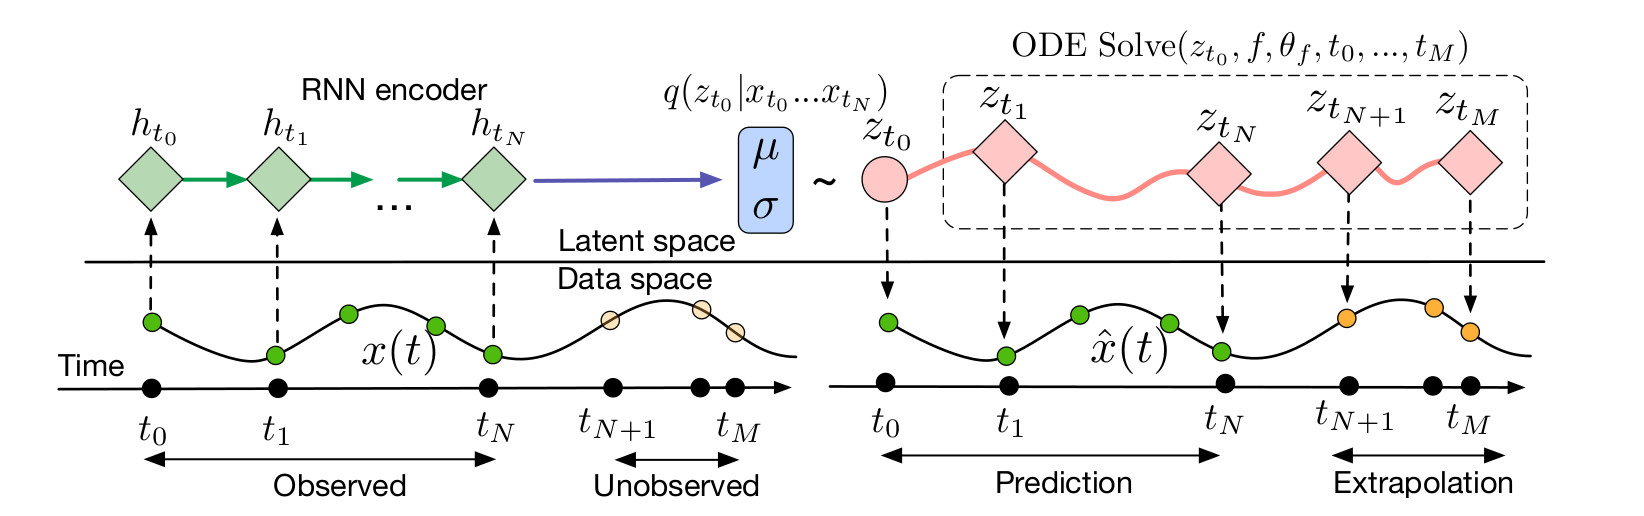
\includegraphics[width=0.9\textwidth]{/home/benjamin/Folders_Python/MVA/MVA_Stage/images/Neural_ODE_01.png}
        \caption{Neural ODE model}
        \label{fig:Neural ODE}
    \end{figure}
\end{frame}

\begin{frame}{Neural ODE - ELBO}
    \begin{itemize}
        \item the stochastic variables are $z_{t_0}$ and the $x_{t_i}$
        \item the joint distribution writes:
            \begin{align}
                p(x_{t_1:t_N}, z_{t_0}) 
                % &= p(z_{t_0})p(x_{t_1:t_N} \vert z_{t_0}) \\
                &= p(z_{t_0}) \prod_{t=1}^{N}p_{\theta_x}(x_{t_i} \vert z_{t_i})
            \end{align}
        \item likelihood:
        \begin{align}
            % p(x_{t_1:t_N}) &= \frac{p(x_{t_1:t_N}, z_{t_0})}{p(z_{t_0} \vert x_{t_1:t_N})} \\
            \log{p(x_{t_1:t_N})} 
            % &= \mathbb{E}_{q_{\phi}(z_{t_0} \vert x_{t_1:t_N})} \log{\frac{p(x_{t_1:t_N}, z_{t_0})}{q_{\phi}(z_{t_0}\vert x_{t_1:t_N})}\frac{q_{\phi}(z_{t_0}\vert x_{t_1:t_N})}{p(z_{t_0} \vert x_{t_1:t_N})}} \\
            % \log{p(x_{t_1:t_N})} 
            &\geq \mathbb{E}_{q_{\phi}(z_{t_0} \vert x_{t_1:t_N})} \log{\frac{p(x_{t_1:t_N}, z_{t_0})}{q_{\phi}(z_{t_0}\vert x_{t_1:t_N})}} \\
                % &= \mathbb{E}_{q_{\phi}(z_{t_0} \vert x_{t_1:t_N})} \log{\frac{p(z_{t_0}) \prod_{t=1}^{N}p_{\theta_x}(x_{t_i} \vert z_{t_i})}{q_{\phi}(z_{t_0}\vert x_{t_1:t_N})}} \\
                &= \sum_{i=1}^{N} \mathbb{E}_{q_{\phi}(z_{t_0} \vert x_{t_1:t_N})} \log{p_{\theta_x}(x_{t_i} \vert z_{t_i})} - \mathbb{KL}(q_{\phi}(z_{t_0} \vert x_{t_1:t_N}) \vert\vert p(z_{t_0}))
        \end{align}
        \item Need to compute the gradients of $\log{p_{\theta_x}(x_{t_i} \vert z_{t_i})}$ w.r.t. $\theta_f$. 
        Methods are forward sensivity, backpropragation through \gls{ode} solver, or \textbf{adjoint sensitivity method}.
        (see \cite{pontriagin_mathematical_2018}, \cite{sengupta_efficient_2014}).
        % \ref{sec:adjoint_sensitivity_method}.
    \end{itemize}
\end{frame}

% A limitation of this model is the assumption that the prior is "concentrated" in the initial value $z_{t_0}$, and that the 
% remaining latent variables are deterministically determined.
% \end{frame}

\begin{frame}{Neural SDE}
    Neural SDE
\end{frame}